\section{Evaluation}
\label{SEC:evaluation}

In this evaluation we set out to answer the following questions using both
the qualitative and quantitative data collected during our study.

\begin{enumerate}

\item Are users able to effectively find bugs using CrashSimulator?  How
does CrashSimulator compare to other tools in this area?

\item Does CrashSimulator allow users to test the areas of
applications in which they are interested?  Are other tools better able to
evaluate these areas?

\item Does CrashSimulator allow its users to construct a test suite
efficiently?  How does CrashSimulator compare to similar tools
efficiency wise?

\item Does user experience level have an impact on tool experience?  Is
there a difference in the skillsets required in order to be effective
with CrashSimulator vs the other tools?

\item Does CrashSimulator provide output that is useful in locating and
fixing bugs?

\end{enumerate}

\subsection{Study Design}

\preston{This is where the study design will go once I've come nailed it
down}

 % Limitation -> Will users be able to identify what caused the problematic
% system call sequence -> Add this to evaluation*

Our goal with this work was to gain an understanding of
how CrashSimulator's
user experience compares to that of other tools and techniques available to
developers.  Because CrashSimulator is able to to test a wide domain
of operations that an
application can perform, we felt it necessary to compare
it with two separate
tools, one in which the test was based on files and one for which the tests
were based on network
activity.  Specifically, we used AFL and Mutiny...


\subsection{Method}

We gathered a group of YYYY participants from a computer science master's
program.  These students had varying backgrounds in relation to software
development and automated testing.  All received AAA hours
of education on each of these tools.  This education focused on the tools'
initial setup, configuration, usage, and how to interpret the tools'
results.  BBB of the students had used AFL in previous course work.  None
of the students had previous experience with Mutiny or CrashSimulator.

% Talk about the challenges around getting a bug fixed,  finding teh source,
% convincing maintainers to take a look, all that.
We asked our participants
to test popular real-world applications with the goal of identifying
new bugs and reporting them to the application's developers.  In performing
this task our participants had to correctly set up and configure each of
the tools, execute a testing process, evaluate the results, and produce
sufficient proof of validity for each bug that a convincing case
could be made for fixing
it.  Each of these steps is an opportunity to for gain insight
into how CrashSimulator stacks up against other tools.

We used three techniques to capture the
experience of our participants as they
used tool.  First, we examined the time required for participants to carry
out defined tasks relevant to the process of bug hunting. This provided a
quantitative measure that was determined by the time
required for participants to
perform each step of the process of finding and reporting a
bug.
We also captured hard counts of the number of bugs identified by our
participants using each of the tools.
The specifics of these bugs will be discussed in more
detail......

For Qualitative concerns, we used surveys to gather participant impressions
on the tools.
These surveys were structured to give insight into how
CrashSimulator compares to the other tools in three areas:

\begin{itemize}

\item Usability of the tool. (i.e. set up, configuration, executing tests,
interpretring results)

\item Extendability of the tool through the creation of additional
anomalies

\item Effectiveness of the tool in its ability to test specific areas of
interest in an application.

\end{itemize}

Additionally, we asked our participants to rate their own experience level in
software development, software testing, and operating systems concepts so
that we might determine whether or not an individual's background has an
effect on what tools they prefer.

\subsection{Are users able to effectively find bugs using CrashSimulator?}

For any of the testing tools used the primary concern is whether or not it
can find bugs.  To evaluate this concern in the case of CrashSimulator,
case we need to answer users are able to
effectively find bugs using the tool....


\subsubsection{Findings}

Table 1 contains counts of bugs identified during the study
broken down by the tool used to
identify them, as well as developer's self reported developer experience
level with operating
system concepts. A total of !!!!15!!!! bugs were found using
CrashSimulator, with the majority reported by participants with a
self-reported high degree of operating system experience.  Participants
with a moderate and low degrees of operating systems experience found more
bugs AFL.....

\begin{figure}[t]
  \center{}
  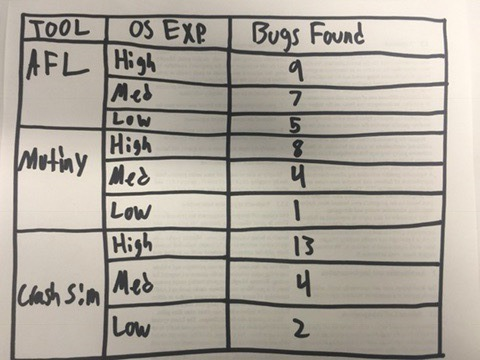
\includegraphics[scale=.5]{images/table1}
  \caption{\emph{Bugs Found by Tool and Experience Level}}
  \label{fig-tool-exp}
\end{figure}


\subsubsection{Discussion}

The above results indicate that, when it comes to using CrashSimulator,
having experience with operating systems concepts is very beneficial...
That said, users with a self-reported low degree of experience with OS
concepts were still able to identify bugs using CrashSimulator's built in
corpus of anomalies and checkers...
Table 2 illustrates which of these checkers were most effective......


\subsubsection{Discussion on Specific Bugs}

!!!! DISCUSSION !!!!


\subsection{How well does CrashSimulator allow users to test the areas of
applications in which they are interested?}

Modern applications typically consist of many different parts (e.g. user
interfaces,  back-end processing, storage, networking) and may require
different skill sets to operate effectively.  These different application
areas also
require disparate testing strategies.  For example, some application
areas such as graphical user interfaces, are notoriously difficult to cover
depending on the tools and techniques being used.  These difficulties
usually result from limitations in the way the testing tool interacts with
the application. We wanted to know whether or not
CrashSimulator was able to effectively test the specific areas of
applications its
users needed to evaluate.  To answer this question, we turn to the
surveys our participants completed regarding their experience with
CrashSimulator.


\subsubsection{Findings}

The results from our surveys indicate that our participants self-reported
backgrounds have an effect on what areas of an application they tested...

Developers with a high degree of experience in software engineering tended
to focus on testing an application's interaction with various library and
operating system provided APIs.  Survery results indicate participants were
satisfied with CrashSimulator's ability to test application's interaction
with file and and network APIs....

Developers with lower self-reported experience
focused more on user interface level concerns...  Preferred AFL's ability
to easily supply a file to be processed to an application....


\subsubsection{Discussion}

Findings indicate that a higher level of software development experience
tends to push participants towards testing interfaces between modules in an
application.  This resulted in overall higher satisfaction with
CrashSimulator amongst participants.....

Users with less self-reported software engineering experience expressed
some concern with CrashSimulator's limitations around testing the user
facing aspects of applications.  For example, CrashSimulator requires more
up front effort than effort than tools like AFL when conducting simple
tests such as mutating the properties of an input file.....


\subsection{Does CrashSimulator allow its users to construct a test suite
efficiently?}

Constructing a test suite using CrashSimulator involves identifying new
anomalies to be tested for and creating the mutators and checkers required
to test an application's response to it.  There is no direct comparison to
this process in AFL...  Mutiny allows users to specify which messages
should be mutated and replayed....


\subsubsection{Findings}

Developers reported a high degree of satisfaction with regard to the speed
of setup for AFL.  Participants felt like CrashSimulator required an
overall higher intitialy outlay of effort before testing could begin.
Additionally, they indicated that expanding a CrashSimulator test suite by
implementing new checkers and mutators was more difficult that either
expanding the scope of fuzzing with AFL or instructing Mutiny to mutate
different messages from a recorded network session.  Participants felt that
CrashSimulator allowed for more specific testing and were pleased with the
ability of CrashSimulator tests to be used across multiple applications
with minimal additional effort once they had been constructed......


\subsubsection{Discussion}

!!!!Discussion!!!!


\subsection{Does CrashSimulator require significant skills to be useful?}

A user's background can dramatically influence their user experience with a
tool.  In answering this question we hope to ascertain whether
CrashSimulator requires its users have significant skills in a particular
area in order to be effective.  Table 2 compares our participants
self-reported skillsets to their positive or negative experiences with
CrashSimulator...


\subsubsection{Findings}

\begin{figure}[t]
  \center{}
  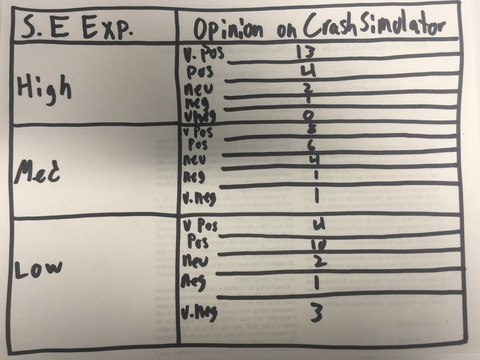
\includegraphics[scale=.5]{images/table2}
  \caption{\emph{Skill Level Compared to User Experience.}}
  \label{fig-skill-exp}
\end{figure}

As can be seen in Table 2, a strong background in operating systems
concepts correlates with a more satisfactory user experience with
CrashSimulator....

Interestingly,  some participants that reported less background in
operating systems had a positive experience with CrashSimulator.  These
participants relied more heavily on built in
anomalies/checkers/mutators....


\subsubsection{Discussion}

Given the level with which CrashSimulator interacts with applications, it
is not surprising that users with significant operating systems backgrounds
are better able to utilize the tool's more advanced features....

It is encouraging to see that users with less os background had success
with the tool.  Based on this, we believe it is likely that CrashSimulator
could be successfully adopted by real-world teams whose members have
diverse background skillsets.  Users that are more comfortable with the
concepts CrashSimulator relies on can supply new testing materials as
needed and other users can rely on CrashSimulators portable nature to use
these tests against new applications without having to worry about their
implementation details.


\subsection{Does CrashSimulator provide output that is useful in locating
and fixing bugs?}


\subsubsection{Findings}

Developer feedback across the board indicated that CrashSimulator's output
made it easier to identify bugs than the simpler crash reports provided by
AFL and Mutiny.  This impression is backed up by the results in Table 3
that show a higher percentage of bugs identified with CrashSimulator were
fixed than bugs identified with the other tools....


\subsubsection{Discussion}

There are two reasons, other than output quality, that bugs found with
CrashSimulator were more likely to be fixed -- bug "depth" and the ease
with which a bug can be fixed.  It is possible that, because CrashSimulator
focuses on a lesser targeted area of an application, more easily fixed, low
hanging fruit style bugs were identified compared to the more battle tested
user input handling codepaths that AFL and Mutiny tend to explore.
Additionally, many of the bugs types identifiable with CrashSimulator arise
because of a minor missing check meaning that the fix is small and easily
incorporated....
